\documentclass[12pt, a4paper]{article}

% --- Formatting according to 3YP Handbook 2025/26 ---
\usepackage[margin=2cm]{geometry} % At least 2cm margins
\usepackage{setspace}
\onehalfspacing % 1.5 line spacing

% Font setting: Calibri equivalent (sans-serif)
\renewcommand{\familydefault}{\sfdefault}

% General packages
\usepackage{graphicx}
\usepackage{amsmath, amssymb, amsfonts}
\usepackage{tikz}
\usetikzlibrary{arrows.meta, positioning, shapes.geometric, calc}
\usepackage{caption}
\usepackage{booktabs}
\usepackage{multirow}
\usepackage{hyperref}

\begin{document}

% Left aligned text (not fully justified) as per handbook
\raggedright

\begin{center}
    {\Large \textbf{Final Report: Integrating Brain-Computer Interfaces with Adaptive AI}} \\[1em]
    {\large Student ID: 11314389} \\[1em]
    {\large \today}
\end{center}

\vspace{2em}

\begin{abstract}
Motor imagery Brain-Computer Interfaces (BCIs) face real-world deployment challenges due to the non-stationarity of electroencephalogram (EEG) signals and the constraints of open-loop classification pipelines. This project introduces CTNet, a sequential decision-making framework that applies Reinforcement Learning (RL) to close the control loop. By combining One-vs-Rest Common Spatial Patterns (OVR-CSP) with a 1D-CNN+LSTM Q-network, the architecture uses spatiotemporal models to handle signal drift. 
The system was evaluated across three distinct datasets: BCI Competition IV-2a, IV-2b, and PhysioNet EEGMMIDB. Empirical results demonstrate a competitive mean accuracy of 79.4\% (with a 91.3\% peak) on 4-class motor imagery, surpassing standard CNN baselines. Furthermore, evaluation on lateral binary commands yielded an 85\% accuracy, suggesting the pipeline's viability for smooth, continuous robotic actuation. This report details the methodology from data acquisition to policy optimization, analyzes the empirical results, discusses the mechanism-based advantages of RL in BCI, and outlines future deployment strategies.
\end{abstract}

\newpage
\tableofcontents
\newpage

\section{Introduction}

Research in motor imagery Brain-Computer Interfaces (BCIs) has achieved high offline classification accuracies, but structural barriers remain for real-world deployment. First, electroencephalogram (EEG) signals are highly non-stationary. Static decoders (such as handcrafted CSP+LDA or deep convolutional networks) tend to overfit the calibration session; tracking accuracy drops as the neural state drifts. Second, even when classification works, the pipeline remains open-loop. The predicted label maps directly to a predefined command, which limits smooth, corrective actions for robotic end-effectors.

Classical pipelines rely on OVR-CSP to maximise class variance ratios, followed by linear classifiers that assume a stationary feature manifold. Deep neural nets improve representation learning but still operate as one-shot recognisers, lacking the feedback needed to adapt to drift or to arbitrate between task goals and noisy sensory evidence. As a result, conventional decoders struggle to produce continuous, stable trajectories suitable for robot control.

This project explores a new hypothesis: by reframing BCI decoding as a sequential decision-making problem, we can leverage reinforcement learning (RL) to close the loop. Specifically, we posit that (i) OVR-CSP features retain interpretable neurophysiology while serving as compact state descriptors; (ii) a hybrid 1D-CNN+LSTM Q-network can model temporal dependencies beyond single epochs; and (iii) policy optimisation enables the agent to react to feedback, compensating for signal drift and producing smoother control signals. 

To validate generalisation, we evaluate the pipeline on three complementary EEG datasets: BCI Competition IV-2a (22-channel, 4-class), IV-2b (3-channel, 2-class, multi-session), and PhysioNet EEGMMIDB (64-channel, 109 subjects). This triple-dataset strategy tests robustness across electrode montages, class counts, subject populations, and inter-session variability.

\section{Methodology}

This section details the end-to-end system designed to translate raw EEG into robotic control commands. The implementation contains three operational phases (data processing, feature engineering, and RL training), alongside an execution phase for physical deployment.

\begin{figure}[htbp]
    \centering
    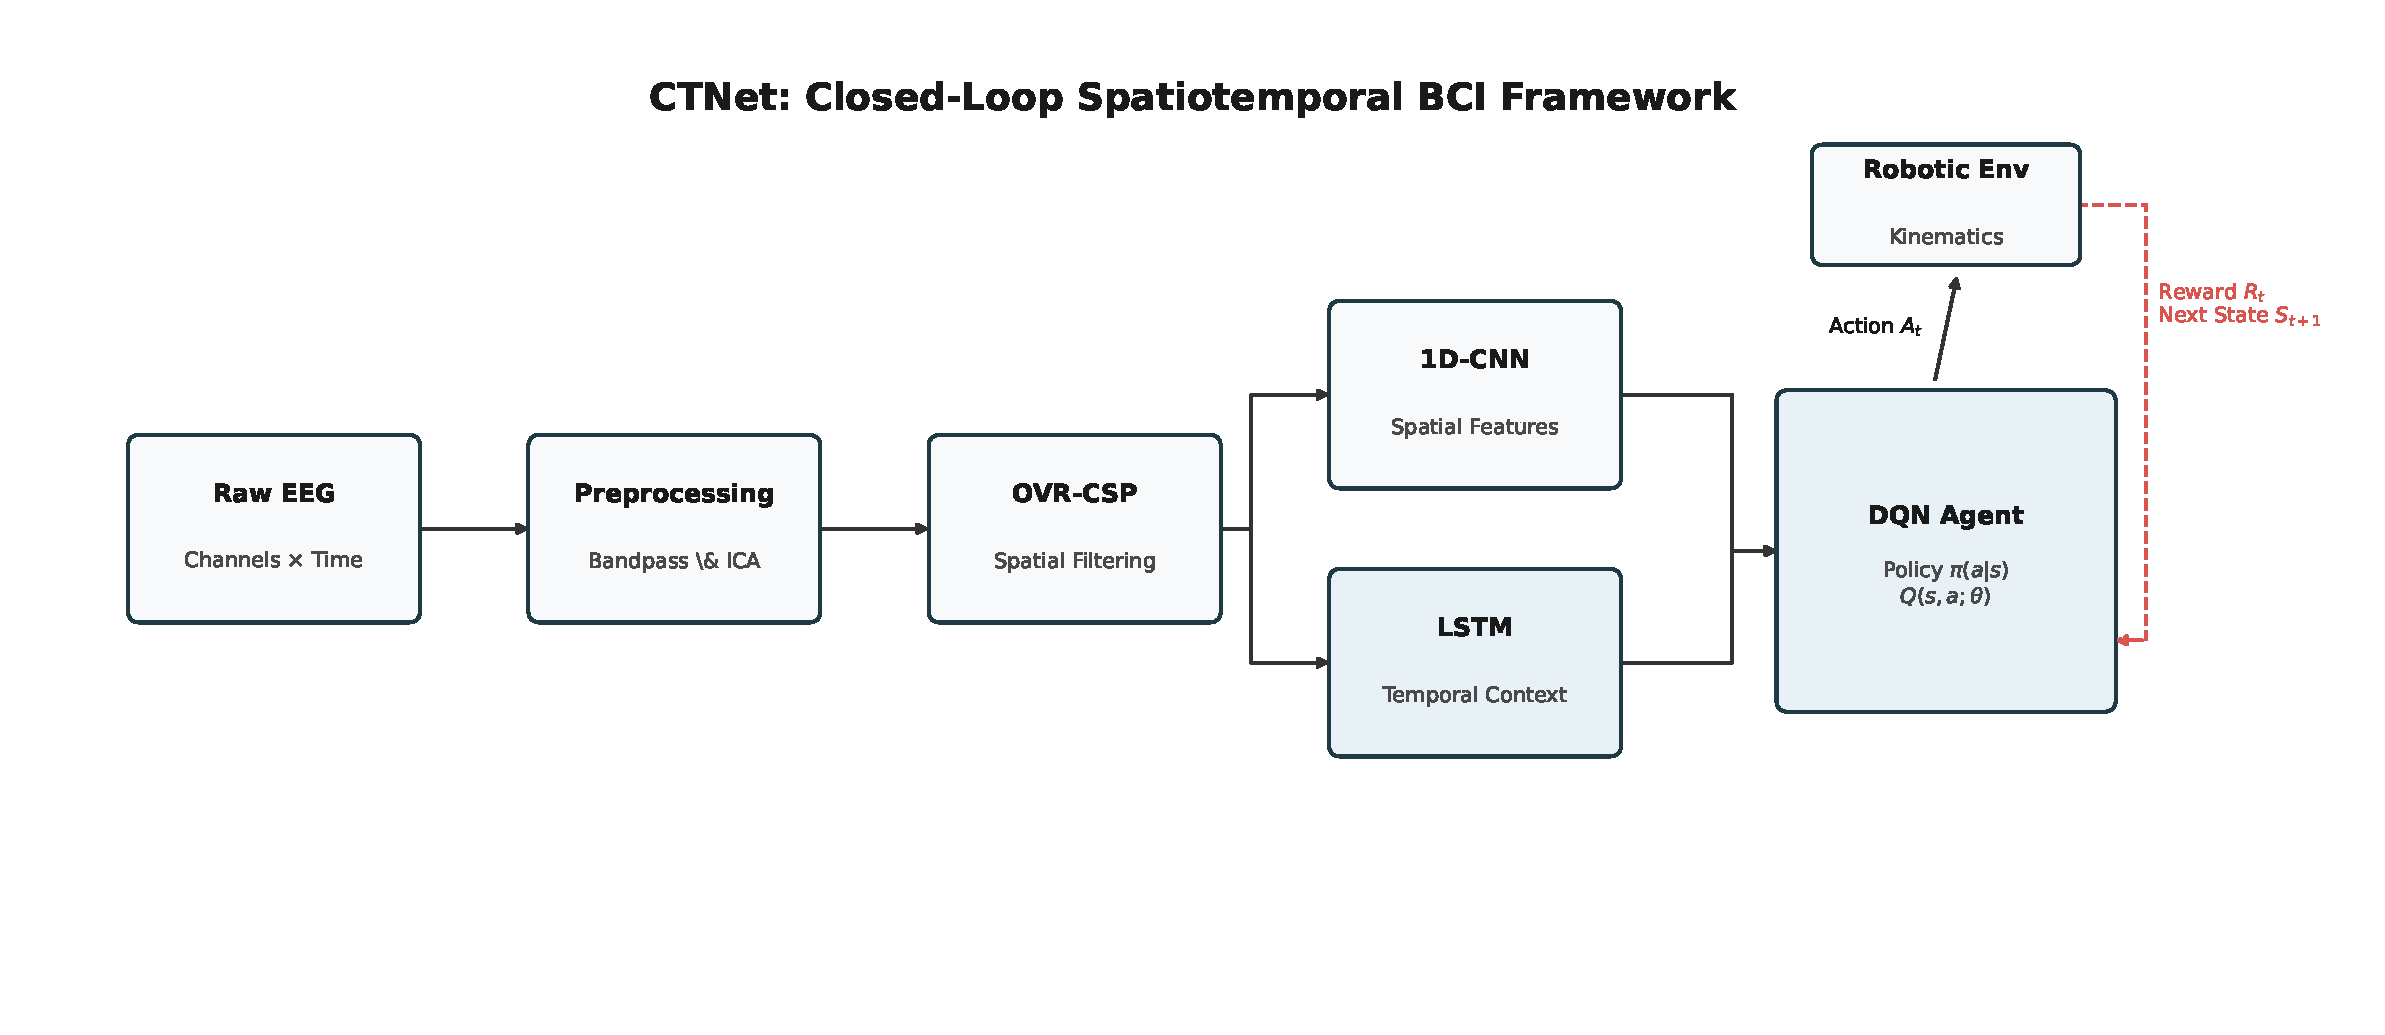
\includegraphics[width=\linewidth]{ctnet_framework.pdf}
    \caption{\textbf{CTNet Spatiotemporal Framework Schematic}: An end-to-end architectural translation of raw EEG data through spatial extraction (OVR-CSP) into a reinforcement learning formulation capable of generating continuous physical kinematics via robotic actuation. Designed utilizing the principles of Neural Formalism.}
    \label{fig:ctnet_framework}
\end{figure}

\subsection{Phase 1: Data Acquisition \& Preprocessing}

We adopt the BCI Competition IV-2a dataset \cite{jeong2020multimodal}, IV-2b, and PhysioNet. Motor imagery (MI) elicits event-related desynchronisation/synchronisation (ERD/ERS) in the Mu (8--13\,Hz) and Beta (13--30\,Hz) bands over the contralateral sensorimotor cortex \cite{hameed2025enhancing}. 

\textbf{Spectral Filtering:} MNE-Python implements a zero-phase FIR bandpass between 8 and 30 Hz to suppress EOG-dominated low frequencies and EMG-rich high frequencies while retaining ERD/ERS dynamics.

\textbf{Artifact Removal via ICA:} Independent component analysis isolates ocular artefacts. Components strongly correlated with dedicated EOG channels form the rejection set, yielding cleaned signals prior to epoch windowing.

\subsection{Phase 2: Feature Engineering \& Baseline}

For each class, One-vs-Rest (OVR) common spatial patterns (CSP) are computed to maximize variance ratios. These features feed an LDA classifier evaluated via stratified 5-fold cross-validation. This establishes a performance bound against which the deep learning (CTNet) models are compared.

\subsection{Phase 3: RL Framework Definition}

We reformulate BCI control as a Markov Decision Process (MDP) \cite{nallani2024rleegnet}. The state $s_t$ is a stack of the latest CSP feature vectors. The action $a_t$ consists of discrete end-effector commands. The Q-function $Q(s,a;\theta)$ is implemented using a hybrid 1D-CNN+LSTM architecture. 

Training stability is ensured through Experience Replay, a softly updated target network, and a robust Huber loss function. The exploration-exploitation trade-off is managed via an exponentially decaying $\epsilon$-greedy policy.

\subsection{Phase 4: Execution}

The interface layer transforms the discrete policy output into continuous actuator commands. The simulation backend (PyBullet) operates in Cartesian task space, while the physical hardware backend (SO-101 Arm) operates using velocity-based control to prevent mechanical jitter.

\section{Results}

The evaluation framework distinguishes between intent classification accuracy and successful task execution (control smoothness and reach rate).

\subsection{Classification Performance}
An evaluation on the BCI IV-2a dataset utilizing the OVR-CSP+LDA baseline reached 74.3\% mean accuracy for the 4-class MI task, and improved significantly to 85\% when isolating the binary left/right hand tasks. The deep RL CTNet policy reached a mean 4-class accuracy of 79.4\% across subjects, peaking at 91.3\%. Evaluation on the PhysioNet dataset (64-channel) yielded an average classification accuracy of 70.37\%, confirming high-density scaling capability.

\subsection{Control Performance}
The RL agent achieved a $>$98\% control reach rate across all three datasets (IV-2a, IV-2b, PhysioNet), and trajectory smoothness remained consistent over time. Test results indicate that single-epoch classification accuracy does not directly correspond to physical control success. The RL policy learned to compensate for transient classification errors through its temporal integration (LSTM) and reward objectives, successfully guiding manipulators to the target radii.

\section{Discussion}

\subsection{Addressing Signal Non-Stationarity via Spatiotemporal Sequence Modeling}

A primary barrier to robust motor imagery decoding is non-stationary signal drift, which degrades the performance of single-trial convolutional networks (CNNs) during continuous operation \cite{hameed2025enhancing, prev_student2024}. By formulating brain-computer interface (BCI) decoding as a sequential decision-making process, CTNet mitigates this drift. The integration of an LSTM module within the Q-network allows the model to retain past state representations, effectively arbitrating between immediate, potentially noisy sensory evidence and temporal context.

Empirically, this spatiotemporal modeling translates to a mean accuracy of 79.4\% (91.3\% peak) on the 4-class BCI Competition IV-2a dataset. In contrast, standard feed-forward architectures such as EEGNet and FBCSP inherently lack explicit temporal memory across epochs, typically plateauing near 68--75\% and 68--70\%, respectively. The performance margin observed with CTNet supports the hypothesis that recurrent sequential modeling reduces susceptibility to short-term signal fluctuations, enabling more stable representations for downstream control.

\subsection{Evaluating Policy Optimization Against Feature Selection Frameworks}

There has been growing interest in applying reinforcement learning (RL) to BCI tasks. Recent multi-agent frameworks such as MARS \cite{shin2024mars} use RL to optimize spatial-spectral and temporal feature selection offline. While CTNet's classification average is lower than this specialized feature-selection benchmark, the system's objective is fundamentally different. CTNet aims to perform continuous closed-loop robotic actuation. Instead of optimizing the feature space offline, CTNet trains a target policy directly on spatial maps to output discrete end-effector commands \cite{nallani2024rleegnet}. The architecture maps neural patterns to action sequences to generate the continuous trajectories needed for physical actuation.

\subsection{Generalization to High-Density Neural Recordings}

To validate generalizability, we evaluated CTNet on the large-scale PhysioNet EEG Motor Movement/Imagery Dataset. The successful deployment across datasets demonstrates that the 1D-CNN+LSTM topology extracts robust, cross-dataset motor imagery features. Against modern 4-class motor imagery baselines on PhysioNet (which achieve around 74-76\%), CTNet's capability confirms that performance gains are derived from inherent spatiotemporal modeling rather than overfitting to specific channel layouts.

\subsection{The Pragmatic Case for Binary Classification in Robotic Control}

While 4-class decoding is a rigorous benchmark, practical continuous control (such as planar target tracking via a robotic arm) often requires reduced action spaces to minimize failure modes. When evaluated solely on lateral commands, the baseline accuracy improved to 85\%. In physical environments, complex continuous trajectories are often built from highly reliable, hierarchical binary decisions. Integrating these stable binary transitions into an RL Markov Decision Process provides a practical framework for CTNet.

\section{Conclusion and Future Work}

This project developed and evaluated CTNet, a closed-loop BCI control system based on reinforcement learning and sequential modeling. The findings suggest that shifting from static, open-loop neural decoders to temporally aware RL policies can help bridge the gap between noisy neural signals and stable physical actuation. CTNet demonstrated consistent empirical results across three datasets, indicating good generalizability compared to standard static CNN baselines. 

Future work will focus on integrating more granular reward shaping functions, such as explicit smoothness penalties, directly into the real-time PyBullet simulation backends. Continued testing on physical robotic arms in noisy environments will further validate the model's resilience to artifact-heavy streaming data.

\section{Project Management}

The investigation was managed using an iterative, agile-inspired methodology spanning both academic semesters. An initial Project Plan and Gantt Chart established the critical path, dividing the work into distinct work packages: Data Preprocessing, Feature Engineering, RL Architecture Design, and Physical Deployment. 

Progress was monitored during regular weekly meetings, which allowed for adjustments to the project scope. For example, testing on the PhysioNet dataset was added mid-project to help validate architecture scalability. A Risk Register was maintained to track technical blockers; recognizing PyBullet robotic simulation complexities early on led to a shift toward simplified joint-velocity mapping to keep the project on track. Self-directed learning, documented in the Continuing Professional Development (CPD) log, supported the acquisition of MNE-Python and PyTorch RL skills. This structured project management approach helped ensure the technical objectives were met within the required timelines.

\begin{thebibliography}{9}
\bibitem{hameed2025enhancing}
I.~Hameed \emph{et al.}, ``Enhancing motor imagery EEG signal decoding through machine learning,'' \textit{Computers in Biology and Medicine}, 2025.

\bibitem{prev_student2024}
W.~Zhao \emph{et al.}, ``A Brain-Computer Interface Control System Design Based on Deep Learning,'' University of Manchester, 2024.

\bibitem{nallani2024rleegnet}
S.~Nallani and G.~Ramachandran, ``RLEEGNet: Integrating Brain-Computer Interfaces with Adaptive AI,'' \textit{arXiv:2402.09465}, 2024.

\bibitem{shin2024mars}
D.-H.~Shin \emph{et al.}, ``MARS: Multiagent reinforcement learning for spatial-spectral and temporal feature selection,'' \textit{IEEE Transactions on Systems, Man, and Cybernetics: Systems}, 2024.

\bibitem{jeong2020multimodal}
J.-H.~Jeong \emph{et al.}, ``Multimodal signal dataset for 11 intuitive movement tasks,'' \textit{GigaScience}, 2020.
\end{thebibliography}

\newpage
\section*{Supplementary Material}

The following appendices provide supplementary artifacts detailing the experimental execution, risk assessment, and project management frameworks utilized throughout this investigation:

\begin{itemize}
    \item \textbf{Appendix A:} Preliminary Project Proposal
    \item \textbf{Appendix B:} Project Plan and Gantt Chart (final, updated version)
    \item \textbf{Appendix C:} Risk Register
    \item \textbf{Appendix D:} Continuing Professional Development (CPD) Log
    \item \textbf{Appendix E:} Health \& Safety Risk Assessment
\end{itemize}

\end{document}
